% Estilo general del documento:
	% Tamaño general:
	
	\documentclass[10pt]{beamer}
\setbeamertemplate{footline}[page number]
	\mode<presentation>{
		\usetheme{Hannover}				% Tema de la presentación.
		\usecolortheme[rgb={0.4, 0.2, 1.0}]{structure} 	% Color principal.
		\setbeamercovered{transparent} 			% Con este comando los ítems ocultos se muestran semitransparentes.
		\useinnertheme{rounded}


	}


	% Mostrar el índice de nuevo al cambiar de sección:
	
	\AtBeginSection{
		\begin{frame}<beamer>{Indice}
			\tableofcontents[currentsection,subsections]
		\end{frame}
	}
	\AtBeginSubsection{
		\begin{frame}<beamer>{Indice}
			\tableofcontents[currentsection, currentsubsection]
		\end{frame}
	}
% Paquetes incluidos por defecto:
	% Tipo de fuente:
	
	\usepackage{palatino}
\usepackage{listings}
\lstset {language=Html, frame=lines, showstringspaces=false}
	% Justificación del texto:
	
	\renewcommand{\raggedright}{\leftskip=0pt \rightskip=0pt plus 0cm} 
	
	% Inclusión de imágenes:
	
	\usepackage{graphicx}
	
	% Matemáticos:

	\usepackage{amsmath, amssymb, latexsym}
	
	% De idioma:
	
	\usepackage[english,spanish]{babel}
	\usepackage[utf8x]{inputenc}
	\usepackage[T1]{fontenc}
	

\title{Videogame analysis}
\author{Jacinto Arias, Adrián Sánchez}
\institute{AI in Videogames \and University of Castilla-La Mancha}
\date{\today}

\begin{document}
\setbeamercolor{background canvas}{bg=black}


\begin{frame}
		\begin{center}
		
\includegraphics[scale=0.3]{logo.jpg} 
		\end{center}
		\titlepage
\end{frame}


\setbeamercolor{background canvas}{bg=white}


	\begin{frame}{Índice}
		\tableofcontents
	\end{frame}

\section{Origins and repercussion}


\begin{frame}{Origins}
	  \begin{itemize}
	   \item Released on 1998 by Blizzard Entertainment.
	   \item Real Time Strategy.
	   \item Standard for this kind of games.
	   \item More than 11 millions of copies have been sold.

	  \end{itemize}

\begin{center}
	  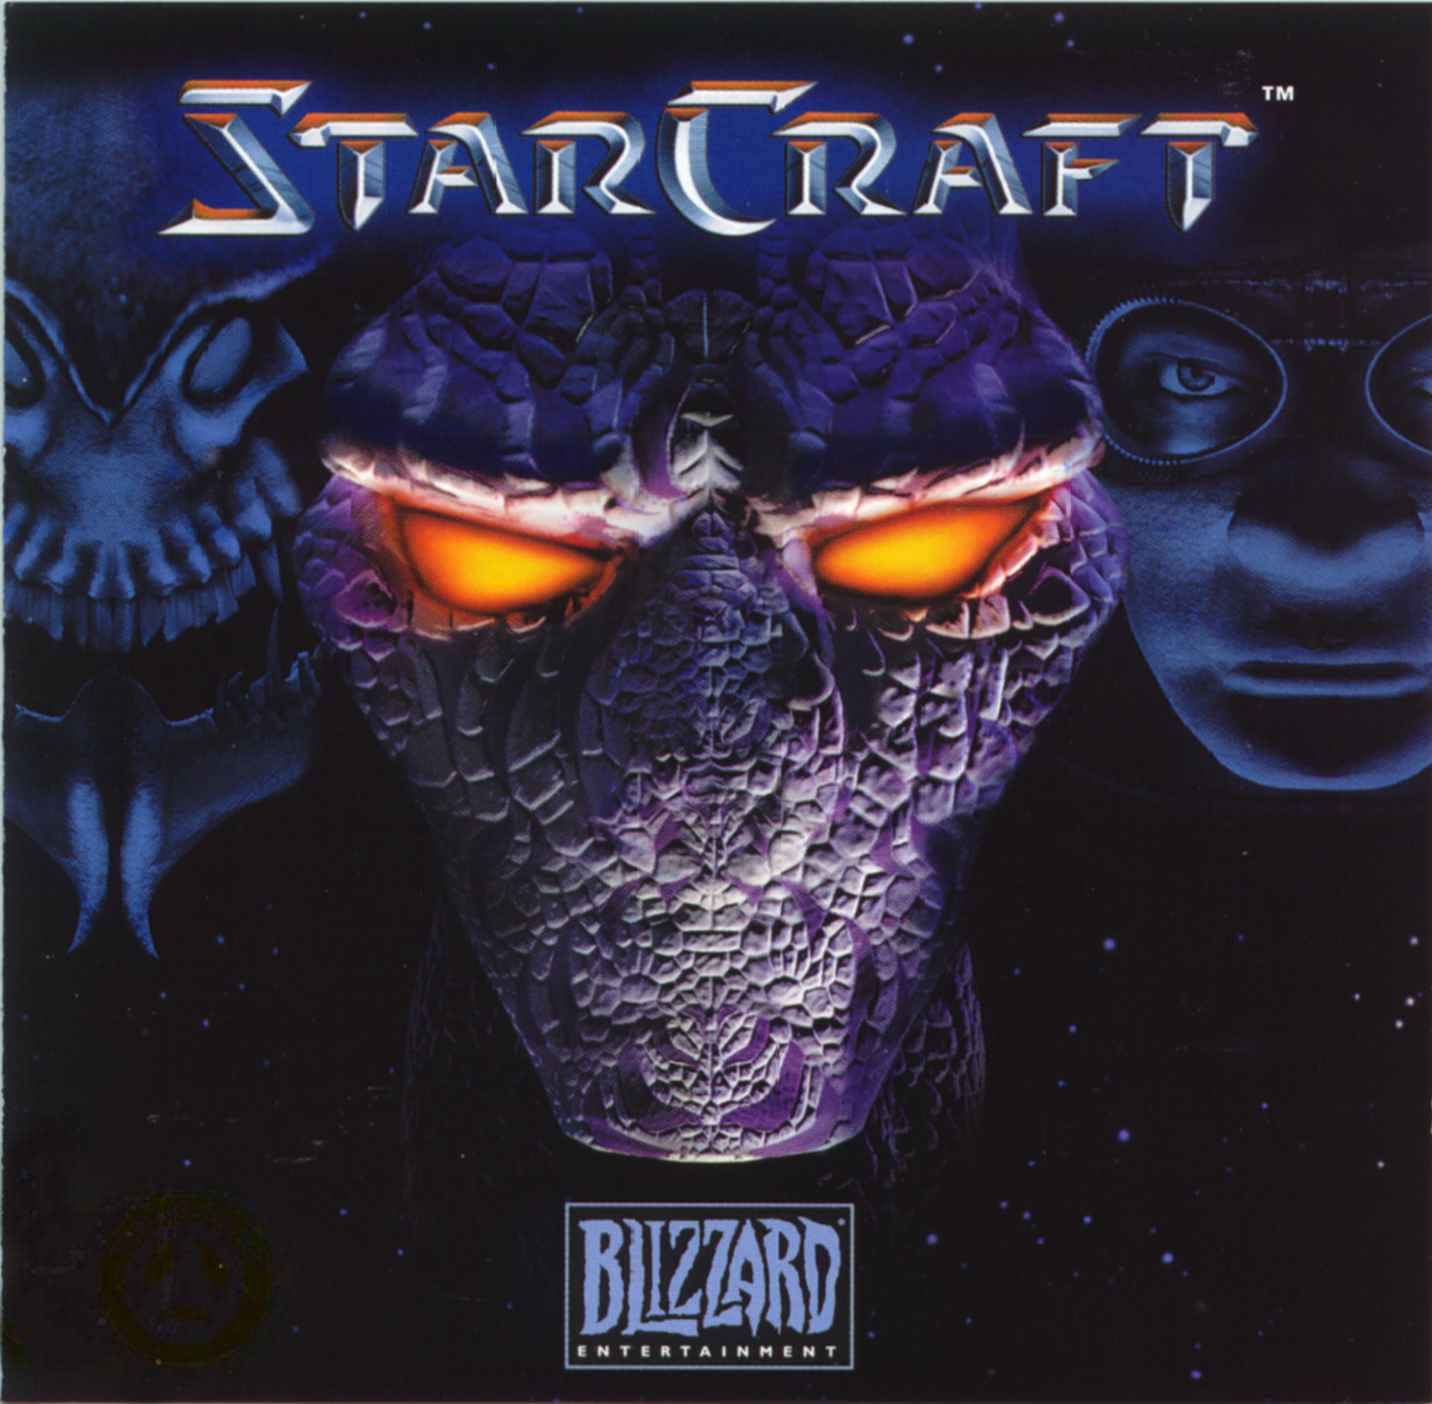
\includegraphics[scale=0.4]{logo1.jpg}\end{center}

\end{frame}


\section{Features and gameplay}

\begin{frame}{The world of Starcraft}

Starcraft is based on a science-fiction world, where three races fight to take control of a solar system far away from the Earth. The three races are:

    \begin{itemize}
     \item \textbf{Terran:} A technological advanced human society that long time ago moved from earth and get lost in space founding a new independent colony.
     \item \textbf{Protoss:} An elder alien race with advanced society and technology that has became in decadency.
     \item \textbf{Zerg Swarm:} An parasitic insectoid race of aggressive lifeforms that consume planets in order to assimilate the genetic of the native ones.
    \end{itemize}

\end{frame}

\begin{frame}{The world of Starcraft}

\begin{center}
	  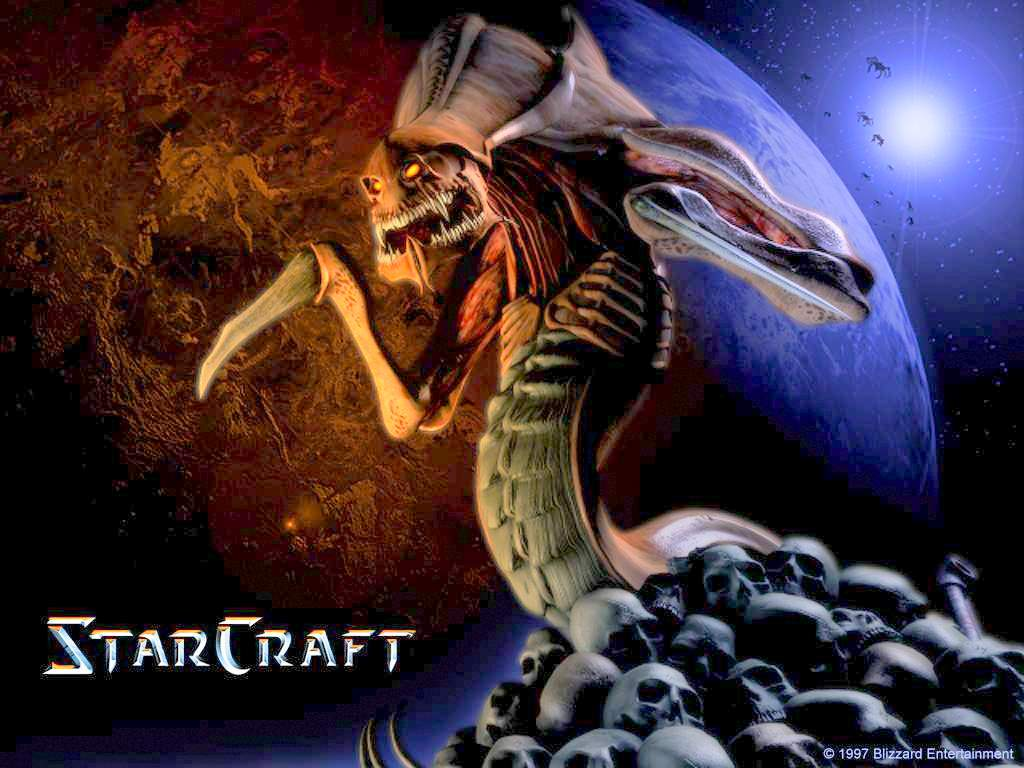
\includegraphics[scale=0.3]{hydralisk.jpg}\end{center}

\end{frame}


\begin{frame}{Game basics}

In order to defeat your opponents you will have to gather resources, build bases and armies and use them against your enemies.

\begin{itemize}
     \item In your screen you will see a portion of the map, you will be able to move along by pushing the screen borders with your mouse.
     \item To control your units and buildings you can select them by pointing with your mouse.
     \item Your units will be able to walk to a different point of the map, to attack other units or patrol some areas.
    \end{itemize}

\end{frame}

\begin{frame}{Game basics}

In Starcraft there are two different kind of games:

    \begin{itemize}
     \item \textbf{Campaign mode}.

    \item \textbf{Multiplayer mode}.
    \end{itemize}

\begin{center}
	  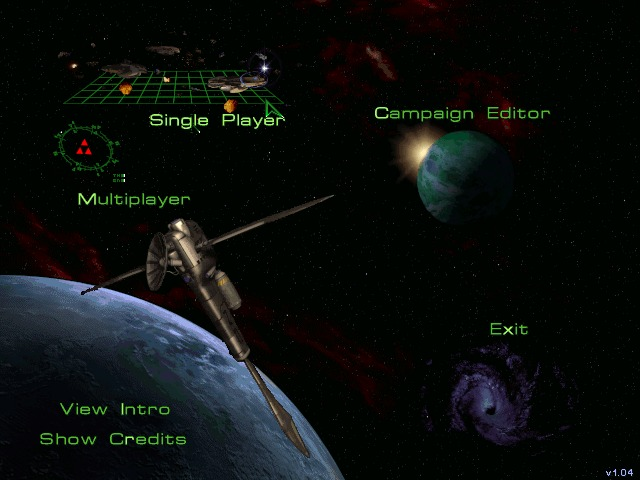
\includegraphics[scale=0.3]{menu.jpg}
\end{center}
\end{frame}







\section{Artificial intelligence principles I: Computational Theory}

\subsection{Game element}
\begin{frame}{Game elements}

In a standard Starcraft game, you will be placed in a map with \textbf{different terrain configurations}.\newline

Also you will find necessary \textbf{resources to gather}.\newline

You will have access to a particular set of \textbf{units} and \textbf{buildings} according to your race, to defeat your opponents.

\begin{center}
	  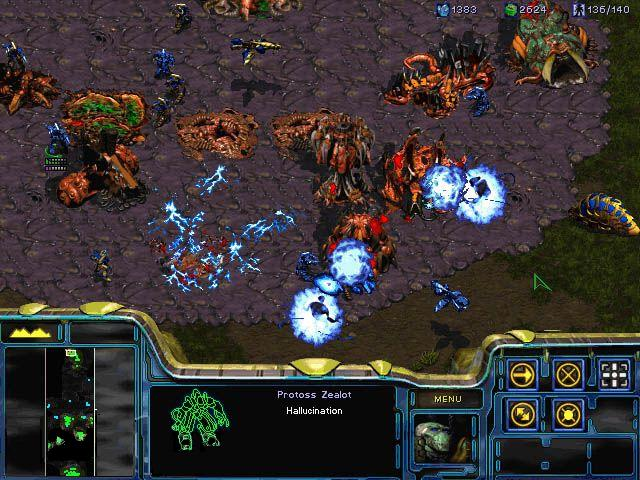
\includegraphics[scale=0.3]{gam1.jpg}
\end{center}
\end{frame}



\begin{frame}{Map, terrain and visibility}

The terrain types condition \textbf{how the units can move around the map}, \small{\textit{i.e a terran marine would walk on the normal ground but it's not allowed to move on the water or lava, however a flying unit will be able to move freely in every type of terrain.}} \newline

Normally, the map is covered in a \textbf{black colour} which represents that you've never visited this area with any unit. Also, there will be areas where the terrain is in a grey colour called \textbf{\textit{war fog}}, so you could not be able to see any of the enemy units in the area, this represents that none of your units can \textit{see} this area.\newline

Each unit has a different \textbf{vision range} which would determine the areas you will see; also, a non flying unit would not be able to see in any terrain higher than the one it is.
\end{frame}


\begin{frame}{Units}

Each race has its set of different units. Every unit in the game has an amount of \textbf{health points}, \textbf{energy}, \textbf{amour} and the majority of them has an \textbf{attack} with its own \textbf{range} and \textbf{damage}. \newline

Each unit is \textbf{stronger} to beat other kinds of units, and is \textbf{weaker} to other kind with no exception, so in order to defeat your enemy you will need to attack him with an optimal army depending of what he has. \newline

Also each race has a \textbf{worker} unit, which is the only unit with can build buildings and gather resources. They are cheap and weak and are the basis of the game economy.
\end{frame}

\begin{frame}{Units}
\begin{center}
	  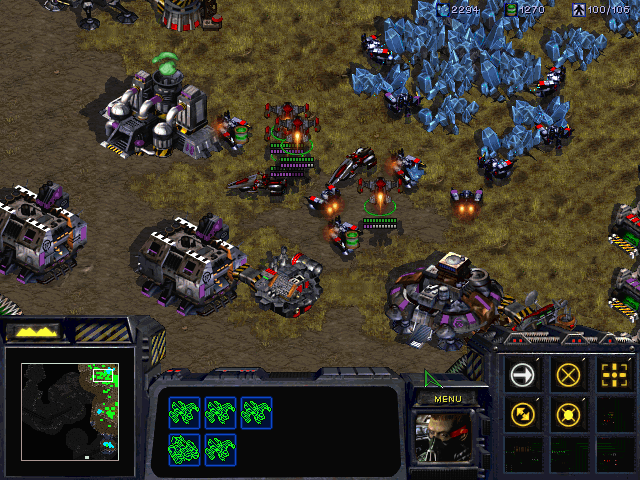
\includegraphics[scale=0.2]{sori.png}
\end{center}
There is two type of units: \textbf{ground} units and \textbf{air} units. The first can only move on the normal terrain and just change to a higher level when using a ramp. \newline

The flying ones could\textbf{ move through every kind of terrain}. \newline

The attack of each unit is defined for ground, air or ground-air targets so it means that some units \textbf{could not be able} to attack specific ones.
\end{frame}


\begin{frame}{Buildings}
A building is like a unit but unlike them are attached to ground and are unmovable and have a great amount of health points. \newline

The buildings purposes include: \textbf{receiving the gathered resources}, \textbf{train units} or do \textbf{researching}. Some structures are \textbf{defensive} so they can attack enemy units.
\end{frame}

\begin{frame}{Resources}
    You will need resources to \textbf{afford} units and buildings.\newline

 Resource is \textbf{gathered} from the map and instantly added to your actual amount. When you build or train units the cost will be \textbf{subtracted} from your amount.\newline

    The game resources are:
    \begin{itemize}
     \item \textbf{Mineral}: most common, gathered from the deposits around the map.
     \item \textbf{Vespene Gas}: less common, it's gathered slowly.
     \item \textbf{Population}: Build special buildings or units to get it. You keep always a maximum level.
    \end{itemize}
\end{frame}

\begin{frame}{Resources}
\begin{center}
	  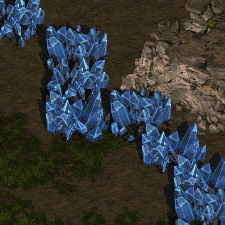
\includegraphics[scale=0.5]{min.jpg}
\end{center}
\begin{center}
	  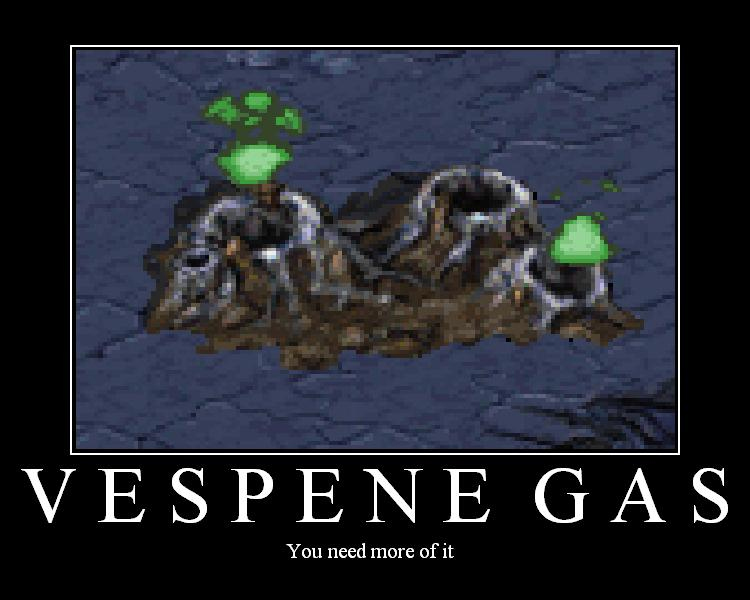
\includegraphics[scale=0.2]{ves.jpg}
\end{center}
\end{frame}

\begin{frame}{Researching and tech tree}
      Each race has an unique \textbf{set of units and buildings}. In order to obtain them the player should meet some \textbf{prerequisites}, commonly it has to build an \textbf{specific building}.\newline

      Some building can do \textbf{researches and upgrades} in order to improve the units or give them a special ability. \newline

Each upgrade costs an amount of resources and takes a lot of time to be completed, but it can \textbf{make a difference} in the game.
\end{frame}

\subsection{Game strategies}


\begin{frame}{Game strategies}
     \begin{itemize}
     \item \textbf{A solid economy is needed.}
     \item \textbf{Exploration is fundamental.}
     \item \textbf{Build your bases to properly defend them.}
     \item \textbf{Harass your enemy and make all the economic damage you can.}
    \end{itemize}
\end{frame}

\subsection{Artificial intelligence applications}

\begin{frame}{Artificial intelligence applications}

\begin{itemize}
 \item Artificial intelligence in the game's core.
 \item Independent behaviour of each unit.
 \item Artificial intelligence as an opponent.
 \item Micro management.
 \item Macro management.
\end{itemize}

\end{frame}

\subsection{Knowledge Extraction}

\begin{frame}{Sources}
As Starcraft is one of the most played games ever, we can find lots of sources were expert discuss about the strategy of the game.
\begin{itemize}
 \item Official Battle.net forums.
 \item Official Blizzard's guides.
 \item Professional teams and fan web pages; searching for ``starcraft strategy'' on google gives more than 17,300,000 results.
\end{itemize}

\end{frame}

\begin{frame} {Economic issues}
	\begin{itemize}
	\item In order to optimally gather resources, you will need 3 workers per deposit.

        \item Keeping large amounts of resources is a bad strategy. You must be able to spend all the resources you gather.

	\item Expand your base once early and keep expanding during the game.

	\item Research every time you can afford it. Researching costs a lot of time and you will get a lot of profit for all the units that you already have.
\end{itemize}
\end{frame}

\begin{frame}{Exploration and map positioning}
     \begin{itemize}
     \item Keep exploring the map from the beginning to the end.
     \item Spy your enemies.
     \item Use the terrain properties.
    \end{itemize}
\end{frame}

\begin{frame}{Follow an optimal construction plan}
 You shouldn't not train or build every type of unit.
 \newline

  You should make a construction plan from the beginning of the game and you should evolve this if the situation require it. 
\newline

The construction plan should be used in order to implement your strategy.
\end{frame}

\begin{frame}{Micro management: attacking}
 By default, a unit will attack the nearest enemy unit.
\newline

  Professional players prefer to direct command their troops to move or attack to specific places or units and they optimize so much their gameplay.
\newline

It's true that a good micro management should win a battle which started in the same conditions.
\newline

    To take advantage of micro controlling on battles, the professional player order their units to focus fire on the strongest units to take them down faster and minimizing the fire that they could inflict to their troops.

\end{frame}

\begin{frame}{Micro management: moving}
  By default, a unit moves on the most straight that it could found to a given point.
\newline

  In order to optimize the movement, the professional players achieve a large numbers of mouse clicks per second in order to smooth the paths that the units follow and avoid the collision between them. 
\end{frame}

\section{Artificial intelligence principles II: Representation and algorithms}

	    \subsection{Application of search techniques}
    
	     
	      \begin{frame}{Path finding}
	      \small
	           \begin{itemize}
		    \item \textbf{Input space:}
		      \begin{itemize}
			 \footnotesize
			 \item The map divided in regions and represented as a non directed graph.
			 \item Each node will be either a passable or an impassable region.
			 \item Actual and desired final location.
		      \end{itemize}
		    \item \textbf{Output space:} The algorithm will return a valid path of the graph.
		    \item \textbf{States:} Each node of the graph. Only the nodes that are passable can be considered as valid states. 
		    \item \textbf{Initial-final state:} The initial location and the desired one.
		    \item \textbf{Operators:} Ramification through states should be done by moving directly to the neighbours of the current node.
		    \item \textbf{Function of heuristic evaluation:} The cost of going from the origin to the destination without considering the condition of the regions.
		   \end{itemize}
	      \end{frame}

	      \begin{frame}{Construction plan optimization}
	      \small
	           \begin{itemize}
		    \item \textbf{Input space:}
		      \begin{itemize}
			 \footnotesize
			 \item The enemy units that you have been discovered.
			 \item The topology of the map.
			 \item You current construction plan (which is a vector containing elements (units)).
		      \end{itemize}
		    \item \textbf{Output space:} A modified construction plan.
		    \item \textbf{States:} Possible construction plans. 
		    \item \textbf{Initial-final state:} A factible final state is when you stop the search by depth.
		    \item \textbf{Operators:} Ramification through states should be adding or deleting elements from the construction plan.
		    \item \textbf{Function of heuristic evaluation:} A numeric weight for a statistic fight between the two simulated armies. A good variation would be a min-max algorithm.
		   \end{itemize}
	      \end{frame}

\subsection{Application of RBS}

\begin{frame}{Deciding a good construction plan}

    The original AI of this game was implemented by using rules.
    \newline

    In order to determine which is the next unit to build. Using the extracted knowledge there will be so potential rules to be constructed. The prototype is IF you se some type of enemy unit THEN build its counter-unit. For example:

    \begin{itemize}
     \item IF you see mutalisk THEN build marines.
     \item IF you see tanks THEN build guardians.
     \item IF you see carriers THEN build ghosts and spectres.
     \item IF you see scouts THEN build goliaths.
    \end{itemize}
 
\end{frame}

\subsection{Application of CBS}

\begin{frame}{Deciding strategies}
 CBS can be applied like RBS but its possibilities are greater.
\newline

By using cases, we can decide not only a construction plan based on our observations but also on the enemy behaviour. You can consult your memory in order to determine if there is a special counter-strategy in order to take your enemy down.
\newline

Also, if you loose by a new strategy that you've never seen before you can store it and use ir in another similar situation. This kind of reasoning is really similar to the one used by human player of this game.
\end{frame}

\subsection{ANN and evolutionary computation}

\begin{frame}{About learning and evolving}
 
There would be a nice exercise to confront many AI controlled opponent in millions of simulated matches having set before a ANN or a evolutionary computation learning process in order to see how far they can reach in their gameplay.
\newline

The fact is that, probably they would play the game at a good level, but when they would be faced against human players, the last ones would quickly get used to them and the machines wouldn't adapt so fast to that new situation. And so starcraft is a commercial game designed mostly to play human vs human, sure that this would never be a priority for the enterprise.
\newline

However some researchers around the world have created AIs to play this game, and when they face it against each other, they could pass the Turing test.
\end{frame}

\subsection{Cooperative behaviour}

\begin{frame}{Cooperative behaviour}
 Some cooperative behaviour can be seen between AI opponents in the current game. But the communications are so poor and their coordination is very bad.
\newline


 They most perform attacks at the same time, but not coordinated, and neither they defend each other or share resources.
\newline

 Implementing an agent based communication between two starcraft AI opponents wouldn't be a hard task if they just pass some trivial information, but this information would be useful for the rest of techniques that can be implemented. 
\end{frame}

\section{Artificial intelligence principles III: Implementation}

  \begin{frame}{API}
   There is an open API to program AI opponent that is used by all the researchers in the competitions of this kind.
\newline

http://code.google.com/p/bwapi/
  \end{frame}


\begin{frame}{The end.}

Thank you for your attention. \newline

	  \begin{center}
	  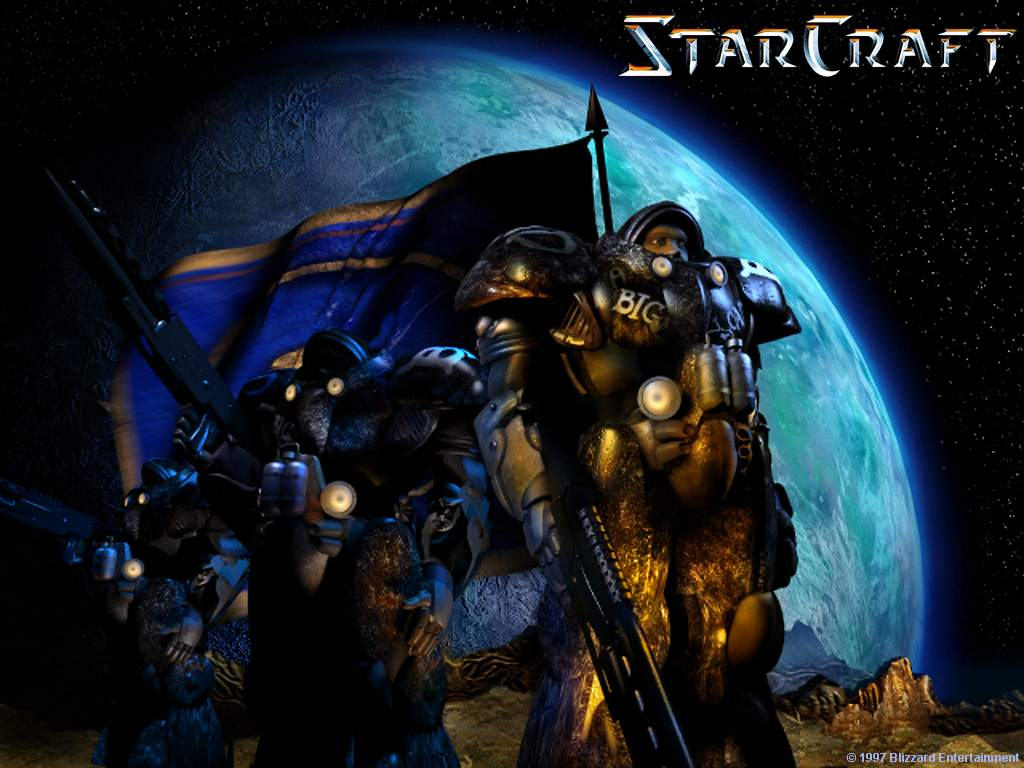
\includegraphics[scale=0.2]{win.jpg}
	  \end{center}


\end{frame}
\end{document}
